%%%%%%%%%%%%%%%%%%%%%%%%%%%%%%%%%%%%%%%%%
% Large Colored Title Article
% LaTeX Template
% Version 1.1 (25/11/12)
%
% This template has been downloaded from:
% http://www.LaTeXTemplates.com
%
% Original author:
% Frits Wenneker (http://www.howtotex.com)
%
% License:
% CC BY-NC-SA 3.0 (http://creativecommons.org/licenses/by-nc-sa/3.0/)
%
%%%%%%%%%%%%%%%%%%%%%%%%%%%%%%%%%%%%%%%%%

%----------------------------------------------------------------------------------------
%	PACKAGES AND OTHER DOCUMENT CONFIGURATIONS
%----------------------------------------------------------------------------------------

\documentclass[DIV=calc, paper=a4, fontsize=10pt, twocolumn]{scrartcl}\usepackage[]{graphicx}\usepackage[]{color}
%% maxwidth is the original width if it is less than linewidth
%% otherwise use linewidth (to make sure the graphics do not exceed the margin)
\makeatletter
\def\maxwidth{ %
  \ifdim\Gin@nat@width>\linewidth
    \linewidth
  \else
    \Gin@nat@width
  \fi
}
\makeatother

\definecolor{fgcolor}{rgb}{0.345, 0.345, 0.345}
\newcommand{\hlnum}[1]{\textcolor[rgb]{0.686,0.059,0.569}{#1}}%
\newcommand{\hlstr}[1]{\textcolor[rgb]{0.192,0.494,0.8}{#1}}%
\newcommand{\hlcom}[1]{\textcolor[rgb]{0.678,0.584,0.686}{\textit{#1}}}%
\newcommand{\hlopt}[1]{\textcolor[rgb]{0,0,0}{#1}}%
\newcommand{\hlstd}[1]{\textcolor[rgb]{0.345,0.345,0.345}{#1}}%
\newcommand{\hlkwa}[1]{\textcolor[rgb]{0.161,0.373,0.58}{\textbf{#1}}}%
\newcommand{\hlkwb}[1]{\textcolor[rgb]{0.69,0.353,0.396}{#1}}%
\newcommand{\hlkwc}[1]{\textcolor[rgb]{0.333,0.667,0.333}{#1}}%
\newcommand{\hlkwd}[1]{\textcolor[rgb]{0.737,0.353,0.396}{\textbf{#1}}}%
\let\hlipl\hlkwb

\usepackage{framed}
\makeatletter
\newenvironment{kframe}{%
 \def\at@end@of@kframe{}%
 \ifinner\ifhmode%
  \def\at@end@of@kframe{\end{minipage}}%
  \begin{minipage}{\columnwidth}%
 \fi\fi%
 \def\FrameCommand##1{\hskip\@totalleftmargin \hskip-\fboxsep
 \colorbox{shadecolor}{##1}\hskip-\fboxsep
     % There is no \\@totalrightmargin, so:
     \hskip-\linewidth \hskip-\@totalleftmargin \hskip\columnwidth}%
 \MakeFramed {\advance\hsize-\width
   \@totalleftmargin\z@ \linewidth\hsize
   \@setminipage}}%
 {\par\unskip\endMakeFramed%
 \at@end@of@kframe}
\makeatother

\definecolor{shadecolor}{rgb}{.97, .97, .97}
\definecolor{messagecolor}{rgb}{0, 0, 0}
\definecolor{warningcolor}{rgb}{1, 0, 1}
\definecolor{errorcolor}{rgb}{1, 0, 0}
\newenvironment{knitrout}{}{} % an empty environment to be redefined in TeX

\usepackage{alltt}	 % A4 paper and 11pt font size

\usepackage{lipsum} % Used for inserting dummy 'Lorem ipsum' text into the template
\usepackage{url}
\usepackage{natbib}
\usepackage[english]{babel} % English language/hyphenation
\usepackage[protrusion=true,expansion=true]{microtype} % Better typography
\usepackage{amsmath,amsfonts,amsthm} % Math packages
\usepackage[svgnames]{xcolor} % Enabling colors by their 'svgnames'
\usepackage[hang, small,labelfont=bf,up,textfont=it,up]{caption} % Custom captions under/above floats in tables or figures
\usepackage{booktabs} % Horizontal rules in tables
\usepackage{fix-cm}	 % Custom font sizes - used for the initial letter in the document
\usepackage{natbib}
\usepackage{sectsty} % Enables custom section titles
\allsectionsfont{\usefont{OT1}{phv}{b}{n} \fontsize{12}{12}} % Change the font of all section commands
\usepackage{hyperref}
\usepackage{float}
\usepackage{fancyhdr} % Needed to define custom headers/footers
\pagestyle{fancy} % Enables the custom headers/footers
\usepackage{lastpage} % Used to determine the number of pages in the document (for "Page X of Total")

% Headers - all currently empty
\lhead{}
\chead{\emph{The U.S. Decennial Census Browser}}
\rhead{}

% Footers
\lfoot{}
\cfoot{}
\rfoot{\footnotesize Page \thepage\ of \pageref{LastPage}} % "Page 1 of 2"

\renewcommand{\headrulewidth}{0.0pt} % No header rule
\renewcommand{\footrulewidth}{0.4pt} % Thin footer rule

\usepackage{lettrine} % Package to accentuate the first letter of the text
\newcommand{\initial}[1]{ % Defines the command and style for the first letter
\lettrine[lines=3,lhang=0.3,nindent=0em]{
\color{black}
{\textsf{#1}}}{}}
\usepackage{color}
\definecolor{purple}{rgb}{.4,0,.8}
\newcommand{\hh}[1]{{\color{magenta} #1}}
\newcommand{\st}[1]{{\color{purple} #1}}

%----------------------------------------------------------------------------------------
%	TITLE SECTION
%----------------------------------------------------------------------------------------

\usepackage{titling} % Allows custom title configuration

\newcommand{\HorRule}{\color{black} \rule{\linewidth}{1pt}} % Defines the gold horizontal rule around the title

\pretitle{\vspace{-50pt} \begin{flushleft} \HorRule \fontsize{15}{15} \usefont{OT1}{phv}{b}{n} \color{black} \selectfont} % Horizontal rule before the title

\title{A U.S. Decennial Census Browser Shiny application: Visualizing the African American population over time} % Your article title
 % This should probably reference geomnet. Don't want it to be too long though
\posttitle{\par\end{flushleft}\vskip 0em} % Whitespace under the title

\preauthor{\begin{flushleft}\large \vspace{-.5cm} \usefont{OT1}{phv}{b}{sl} \color{black}} % Author font configuration

\author{Kiegan Rice, } % Your name

\postauthor{\footnotesize \usefont{OT1}{phv}{m}{sl} \color{Black} % Configuration for the institution name
Iowa State University % Your institution

\par\end{flushleft} \vspace{-.5cm} \HorRule \vspace{-1cm}} % Horizontal rule after the title
\date{} % Add a date here if you would like one to appear underneath the title block

%----------------------------------------------------------------------------------------
\IfFileExists{upquote.sty}{\usepackage{upquote}}{}
\begin{document}
%\SweaveOpts{concordance=TRUE}
\setkeys{Gin}{width=0.5\textwidth}


\maketitle % Print the title

\thispagestyle{fancy} % Enabling the custom headers/footers for the first page 

%----------------------------------------------------------------------------------------
%	ABSTRACT
%----------------------------------------------------------------------------------------

% The first character should be within \initial{}
\vspace{-1cm}
%\initial{U}\textbf{sing a new way to visualize network data in \texttt{R} with \texttt{gglot2}, I examine the evolution of the African slave trade from the $16^{th}$ through the $19^{th}$ centuries. \st{XXX I feel like I need more here. Will add more when paper is more fleshed out.}}

%\initial{T}\textbf{he Trans-Atlantic Slave Trade Database, hosted by Emory University, contains information on nearly 35,000 voyages of slave ships from 1514 - 1866 between Europe, Africa, and the Americas. The entire database contains 279 variables with information on the 34,948 voyages. While the website dedicated to this data contains a dashboard to subset and visualize the data, I wanted to view the data in a new way. I use the \texttt{geomnet} package because I wanted to show that the user can visually explore the data in a way that leaves them with a deeper understanding of the structure of the slave trade. I start by visualizing all of the data I pulled from the database on one map, then I look at different subsets of it, and I end with a much deeper understanding of the slave trade and its impact on the world.}
%----------------------------------------------------------------------------------------
%	ARTICLE CONTENTS
%----------------------------------------------------------------------------------------
\section*{Introduction}

\initial{C}ensus data provide an important snapshot of information about a country at different times throughout its history, and their value is difficult to overstate.  While history books present a narrative of the events that occured, students themselves often don't get to interact with the raw data in that learning environment. Clean and accessible census data allow the exploration of different demographic groups over time, or investigations of a particular period of time and what the demographic and economic landscape looked like in the past. Even today, data about the world around us opens a pathway for learning more about places we haven't been and groups of people with whom we may not usually engage.  

\par From an early point in the United States' history, there were many ``eminent men of science" who recognized the value of the census data and worked to aggregate and present those data. Francis A. Walker's ``Statistical Atlas of the United States", based on the 1870 census, was an impressive effort in aggregating population data to present them in a visually appealing way \citep{StatisticalAtlas}. Although the Census Bureau's "Statistical Atlases" eventually stopped being created, they were an important start to the effort of visually presenting census data to a wider public (see~\autoref{atlas}).

\begin{center}
\includegraphics[width=.4\textwidth]{./figures/colored-population-stat-atlas.png}  
\captionof{figure}{A visualization of the African American population in the United States from the ``Statistical Atlas of the United States".}\label{atlas}
\end{center}

\par Today, as methods of data analysis and visualization continue to be developed and improved, access to census data allows us to look back on that history and explore, synthesize, and visualize the information. When aggregated and presented in a clear manner, viewers can learn more about patterns in many different parts of the population. A 2007 paper about the Statistical Atlas discusses just how much information is present in those original charts and demonstrates several other ways of presenting the information that can be found therein \citep{ChartInterview}.  

\par Ever-improving visualization and data-wrangling methods in R \citep{RCoreTeam} give those interested in statistical graphics a wealth of opportunities to explore and learn from data; in particular, incorporating user interactivity using Shiny has revolutionized the way statisticians share and communicate information \citep{Shiny}. However, it is difficult to make use of these tools with census data if those data are not available and easy to explore in one location.  

\par An inherent problem in census data is that a country's census changes over time; the variables collected, how they are collected, and even the locations on which they are collected are updated as the country is formed, and subsequently grows and changes. The United States census data are no exception to this rule. In little under two and a half centuries, the census has taken many different forms. Data on occupations have transformed as the employment landscape has changed; new states have been formed, the most recent being within the last 100 years; definitions of various demographic groups and the terminology used to describe them have been updated as the demographic makeup of the country has changed. Each decennial census brings a different set of variables to the table. Sometimes these variables are new things the Census Bureau is interested in learning about, while sometimes they remove variables that are no longer relevant or whose information is captured elsewhere.  

\par Unfortunately, because the founders of the U.S. Census were unable to see 200 years into the future, those interested in working with census data are left with quite the inescapable mess. If you want to focus in on a particular demographic group and their journey as part of the population of the United States, you may have ten or more different variable names to describe that one group over the course of the census from 1790 to 1960 - and that is just for a single group! Of course, we cannot just simply change variable names to match our own research needs. It is important to keep the data in their true form and be respectful of the way in which the population was defined at different times throughout history, even if our instinct may be to `clean' the data by changing variable names.  

\par This, of course, leaves the user with a wide variety of variables that are far from consistent across years. In order to track one demographic group across years - let alone many groups - a clean user interface that helps users see exactly what information is available to them is a necessity. To streamline the process and assist researchers in finding out to what information they have access and what information they lack, a U.S. Decennial Census Browser is presented as a Shiny application, with the ability to explore available variables within a certain year or across several years. Additionally, a Visualization tab will allow users to immediately visualize the variables they have picked across different years to get an initial look before downloading the data in the form of `tidy' comma-separated values (csv) files. 
%------------------------------------------------

\section*{Data Access}

Should I include a small section about Data Access? Or should I condense the introduction and add where the data is coming from in that initial section?  


\section*{The Census Browser Shiny application}  

\par The Shiny application has three main points of focus, split into separate tabs. The first tab, `Single Year', allows users to explore all available variable names for a single year of the decennial census at a time. After choosing a particular year, users can look for up to two specific variables of interest by using two available text search bars. This will narrow down the possible variable names, allowing for a more narrow focus in a given year.  

\par The second tab, for `Multiple Years', brings in the ability to compare availability of variables across several years. Users may select a range of years and, if they so choose, narrow down the given results with a text search term. These results are presented as a table with all chosen years as `columns', while all relevant variable names appear as `rows' in the table. An `X` indicates the presence of that particular variable name in the corresponding year. A totals column to the far right allows users to not only see in how many years each variable appears, but also order the relevant variables by that frequency.  

\begin{center}
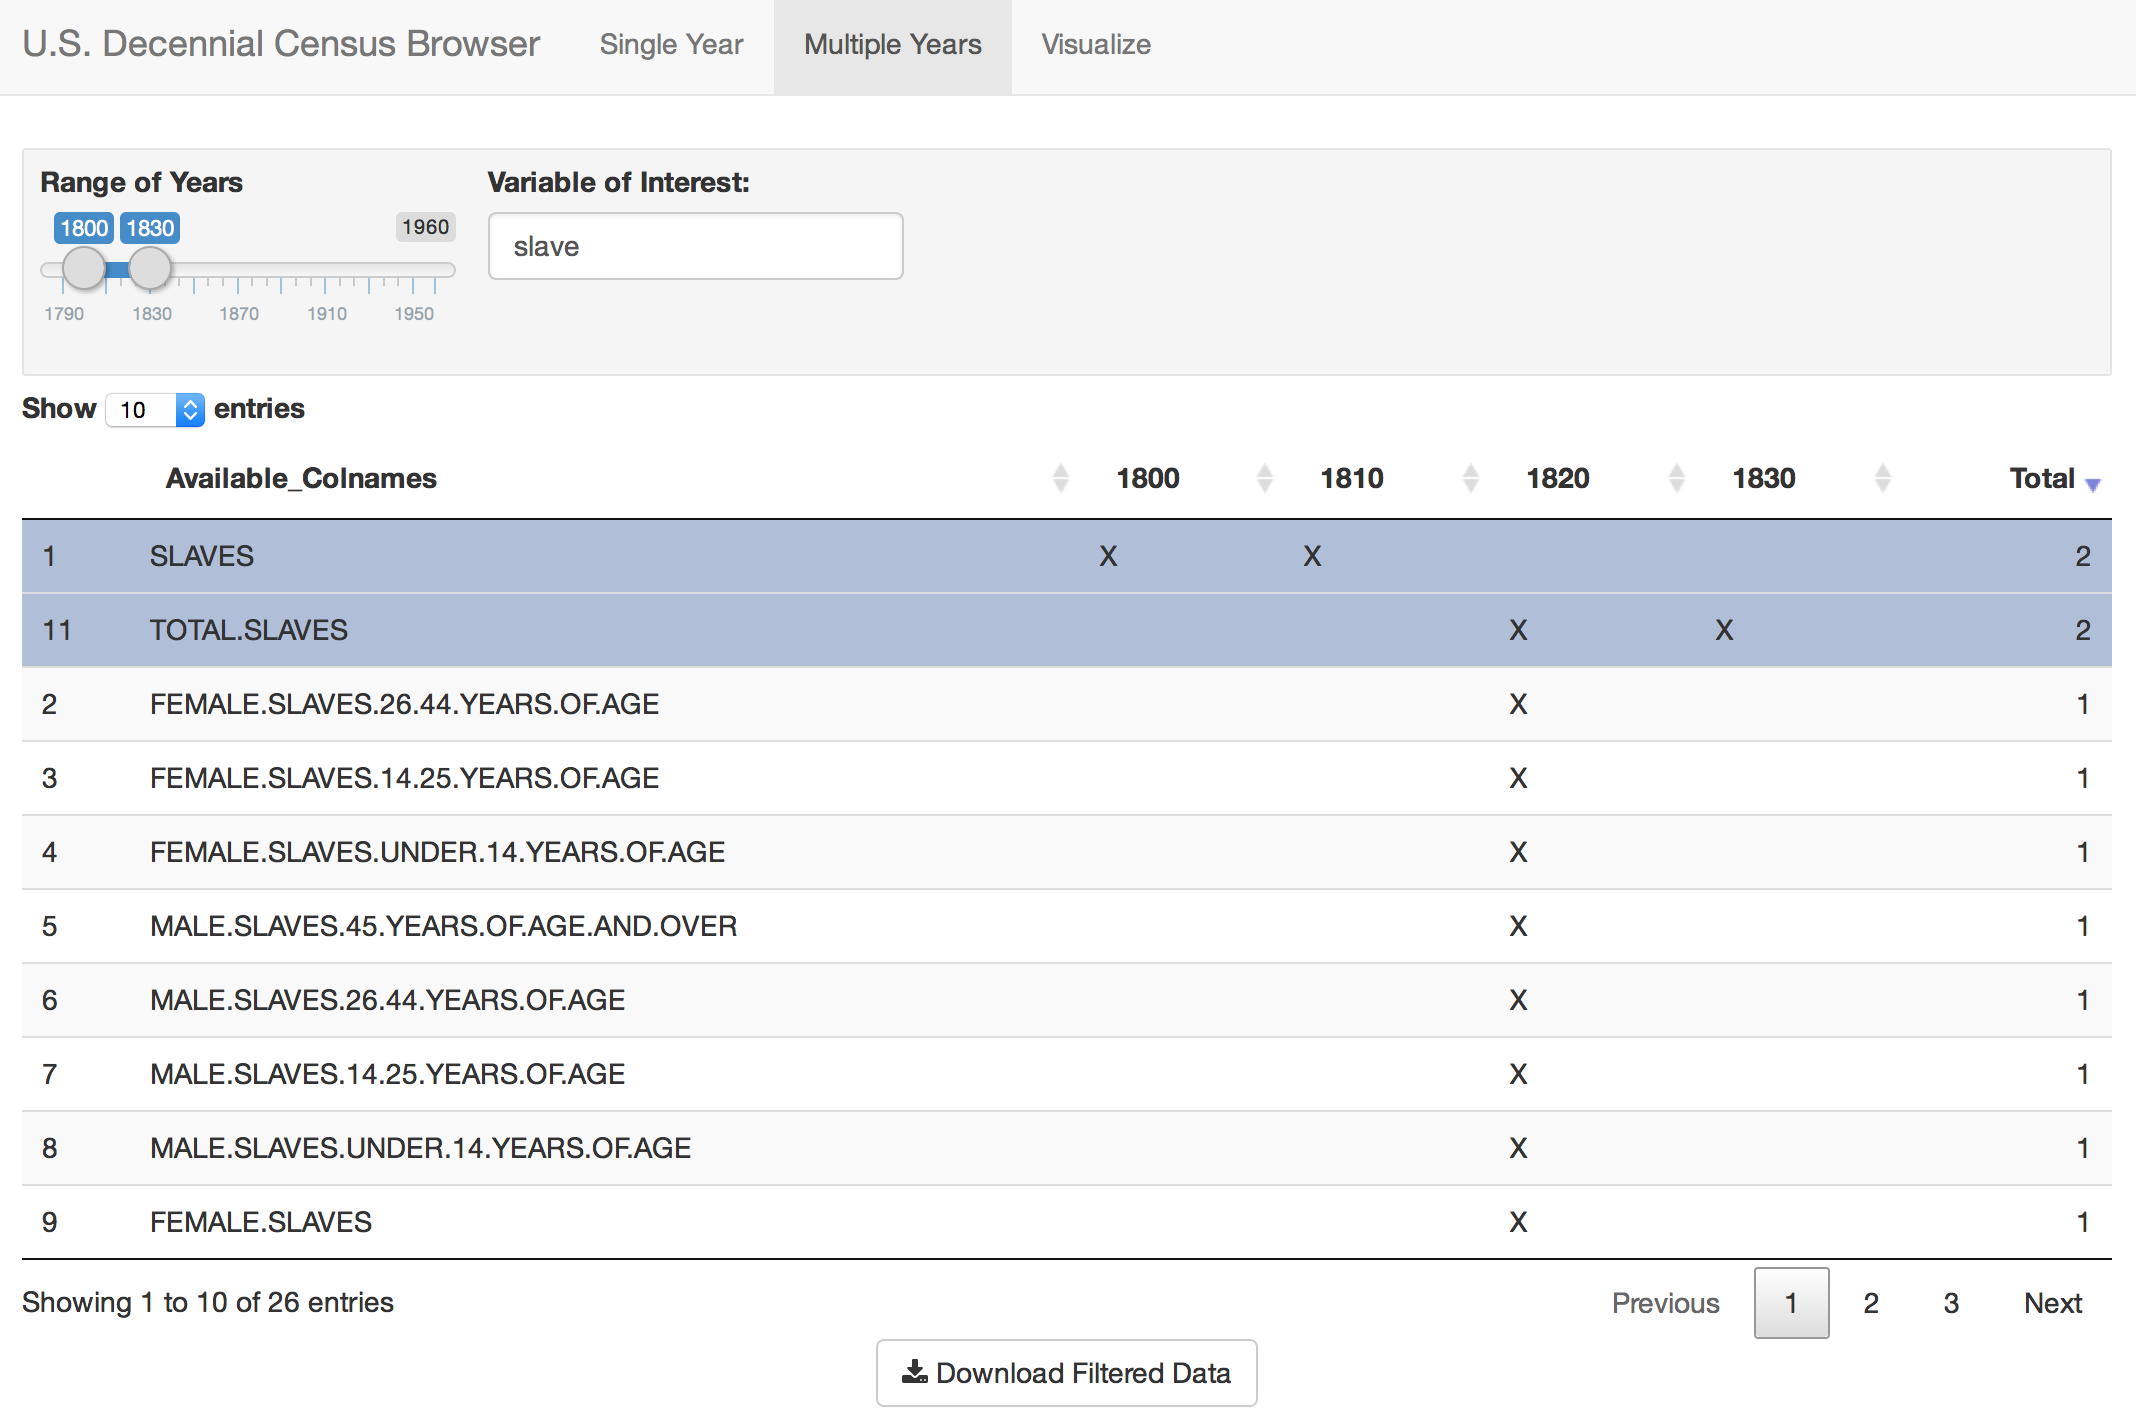
\includegraphics[width=.45\textwidth]{./figures/search_slaves_40years.png}  
\captionof{figure}{Resulting view of the `Multiple Years' tab after restricting the range of years to between 1800 and 1830, and searching for the term `slave'.}\label{shiny_1}
\end{center}

\par The final tab, `Visualize', creates an on-the-spot visual representation of the data selected in the `Multiple Years' portion of the application. Users may choose to simply separate data by year, and sum over all variables chosen within each year, or facet by both year and variable chosen. Depending on the range of years selected by the user and the number of different variables chosen, the latter can easily become a very large grid environment. However, it still allows users to see several things about the particular variables and years they are looking at (see \autoref{shiny_2}).

\begin{center}
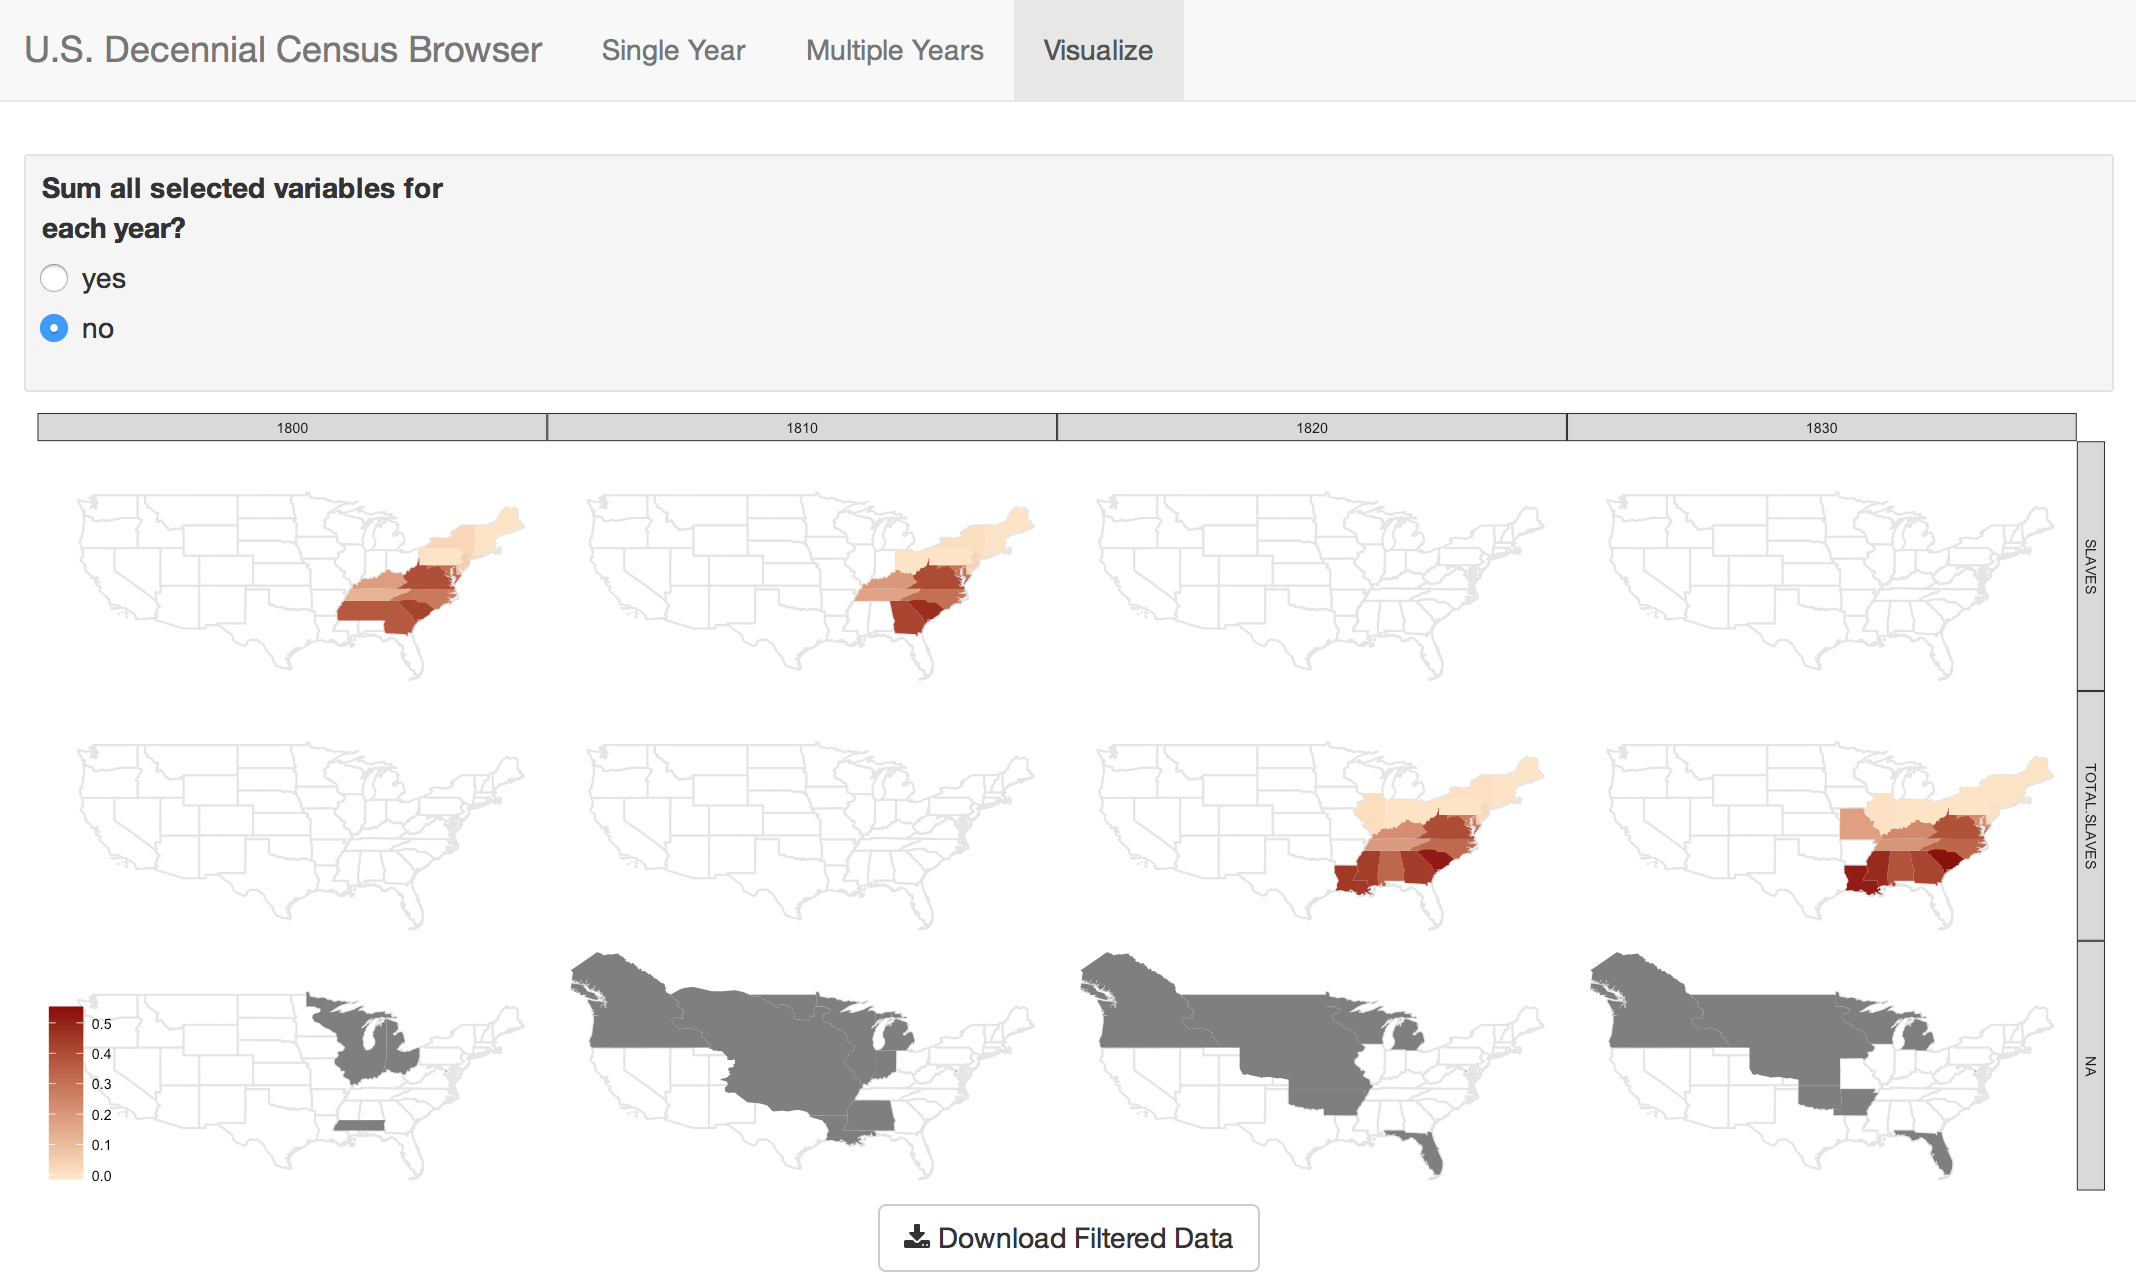
\includegraphics[width=.45\textwidth]{./figures/visualize_slaves_40years.png}  
\captionof{figure}{A visual represenation of available variables for total number of slaves between the years 1790 and 1840, with period-accurate mapping for state boundaries.}\label{shiny_2}
\end{center}

\par First of all, every plot has the outlines of the 48 contiguous states as of 1999. Above that base, the outlines for each state are plotted as they were in the year represented. This means that users can see varying state boundaries across years - however, since these are the areas data were actually collected on at the time, they are the true representation of the geographic regions for the demographic groups chosen. In some years, there are states that still hold Territory status, or are not yet included in the decennial census. These will show up in a bottom row, since they have \texttt{NA} values for the variables. However, it is still useful to see where those boundaries existed and see how they change over time as you pan across the columns.

\par Secondly, users can see how variable names change over time. They can see this during the initial selection of variables in the `Multiple Years' tab; however, now they can see differing variable names for an equivalent or similar demographic group and still directly compare the values on the maps. 

\section*{A Closer Look at the Data}

\par After ordering by how many years each variable appears in, the available variable names show a serious lack of continuity. The four ever-present variables (\texttt{Year}, \texttt{State}, \texttt{TOTAL.POPULATION}, and \texttt{Type}) each appear ten times, once in each year selected. After that, the next most common variable only appears in four of the ten years we have chosen. This highlights some of the hurdles that we will encounter when tracking any demographic group over time. 

\par Since the focus will be on African Americans throughout U.S. history, the first search term needed is \texttt{SLAVE} in the early years of the U.S. census. The vast majority of African Americans were slaves when the United States was founded, so variables that count the number of slaves tell the story about the African American population in early U.S. history. Note that the `SLAVE` categorization is the only term the U.S. census had related to African Americans in the early years of the census, so it is also the only source of information available on that group for that time period.  




\begin{knitrout}
\definecolor{shadecolor}{rgb}{0.969, 0.969, 0.969}\color{fgcolor}\begin{figure}[h]
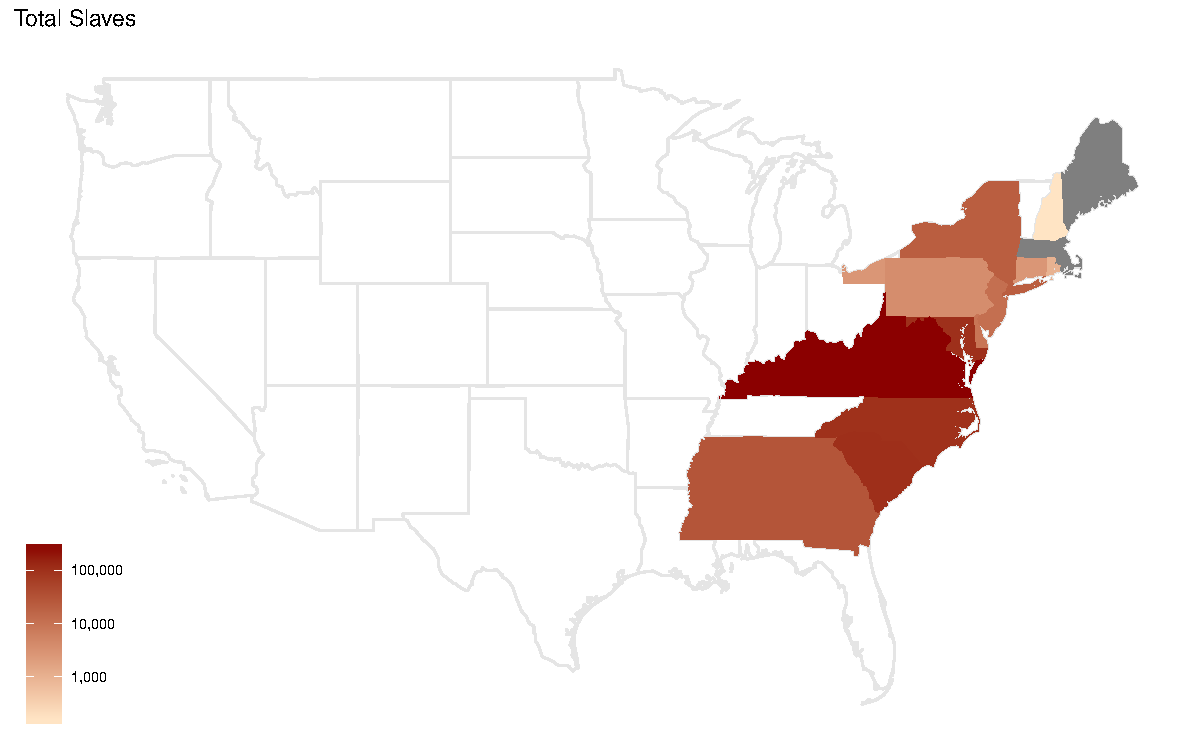
\includegraphics[width=.5\textwidth]{figure/map_1790-1} \caption[Total number of slaves per state in 1790, plotted on a continuous log scale]{Total number of slaves per state in 1790, plotted on a continuous log scale. State boundaries for July 4, 1790 were gathered from `USAboundaries` package.}\label{fig:map_1790}
\end{figure}


\end{knitrout}


With a visualization of the slave population in the United States in 1790 in hand (see \autoref{map_1790}), it is possible to look at subsequent years of the decennial census in a similar manner to see how the population changes over time.  

\begin{knitrout}
\definecolor{shadecolor}{rgb}{0.969, 0.969, 0.969}\color{fgcolor}\begin{figure}[h]
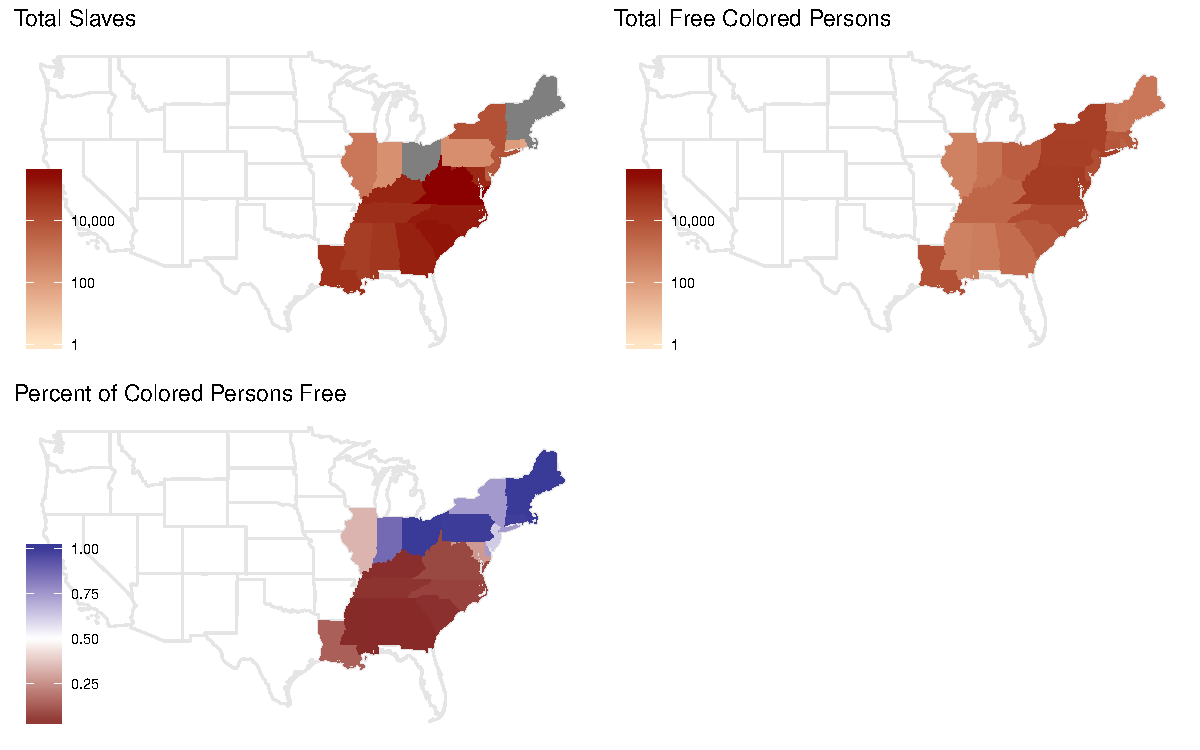
\includegraphics[width=.5\textwidth]{figure/map1820-1} \caption[Total number of slaves, total number of free colored persons, and percentage of colored persons free in each state in 1820 United States]{Total number of slaves, total number of free colored persons, and percentage of colored persons free in each state in 1820 United States.}\label{fig:map1820}
\end{figure}


\end{knitrout}


Jumping to the year 1820, and again filtering on that particular year, we learn new information about the African American population. The census at this time includes a count of \texttt{TOTAL.FREE.COLORED.PERSONS}, as there are citizens who are African American or other minorities that are free, and not slaves. At this time, many minorities were grouped together in the ``colored persons" category, and as before, we do not have any other record for African Americans except this categorization and the ``slaves" categorization. However, since the 1820 census included records for both \texttt{TOTAL.FREE.COLORED.PERSONS} and \texttt{TOTAL.SLAVES}, we can also now visualize the percentage of African Americans in each state that were categorized as "free persons" as opposed to slaves (see \autoref{map_1820}). Knowing that both of these variables are available allows for a powerful comparison by visualizing the growing divide between northern and southern states in the United States at that time.

\begin{knitrout}
\definecolor{shadecolor}{rgb}{0.969, 0.969, 0.969}\color{fgcolor}\begin{figure}[h]
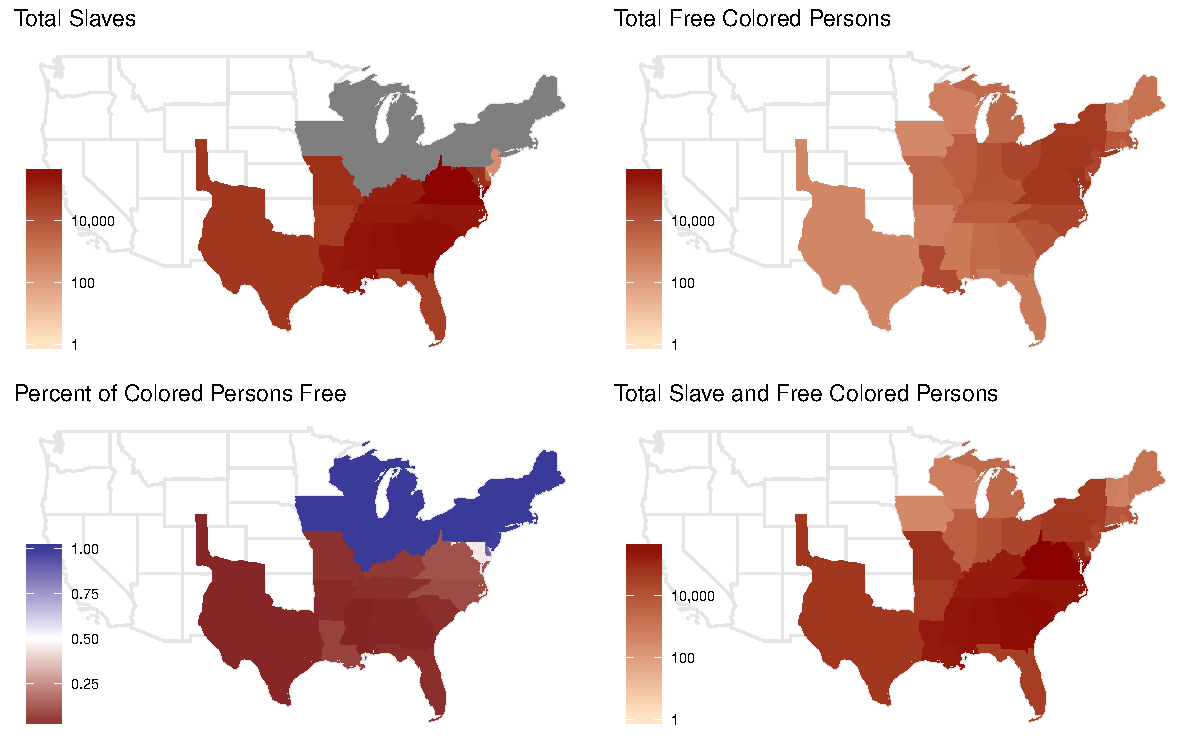
\includegraphics[width=.5\textwidth]{figure/map_1850-1} \caption[Total number of slaves, total number of free colored persons, and percentage of colored persons free in each state in 1850 United States]{Total number of slaves, total number of free colored persons, and percentage of colored persons free in each state in 1850 United States.}\label{fig:map_1850}
\end{figure}


\end{knitrout}

Moving forward in time, even more information can be gleaned about this population. When we subset on the year 1850, we see that although there is still a \texttt{TOTAL.SLAVES} column in the record, many states no longer record this variable; by then, they had already abolished slavery. We can transform these \texttt{NA} values into zeros to account for this difference in the data and allow us to still calculate the percentages of free African Americans. Starting in 1850, we can also start investigating what the total African American population looks like in each state, beyond just the size of the slave population and freed population (see \autoref{map_1850}).

\begin{knitrout}
\definecolor{shadecolor}{rgb}{0.969, 0.969, 0.969}\color{fgcolor}\begin{figure}[h]
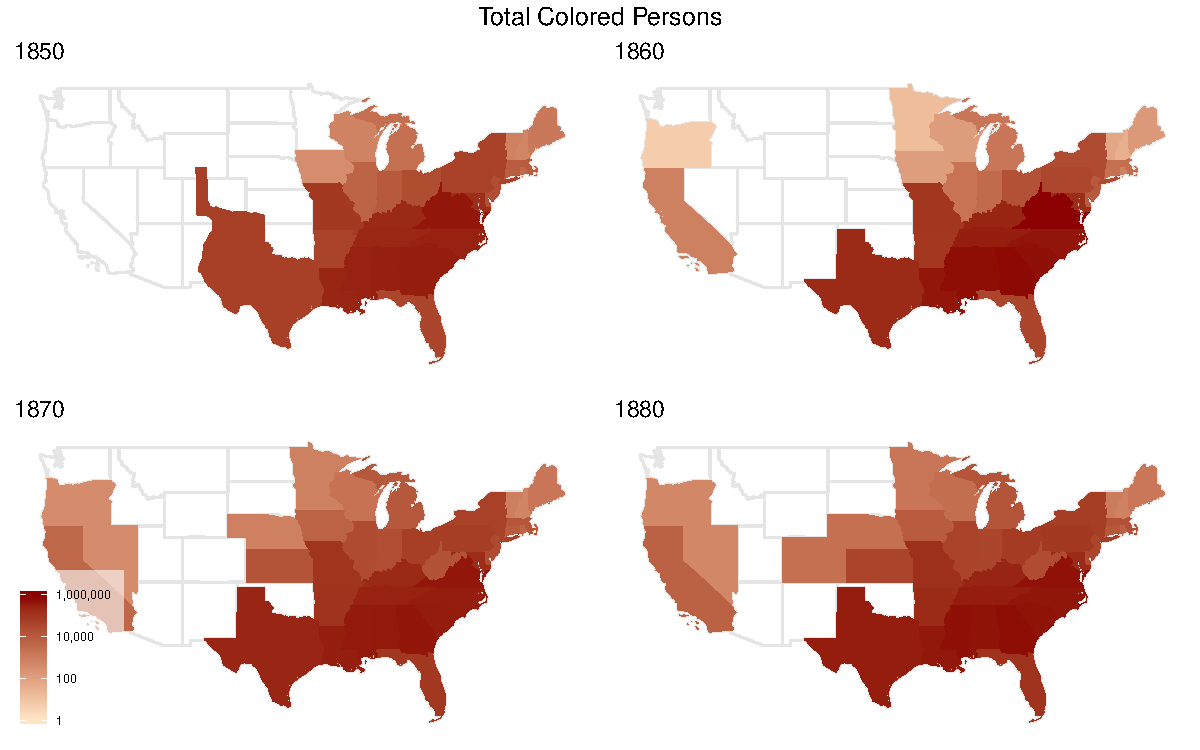
\includegraphics[width=.5\textwidth]{figure/map_1800s-1} \caption[Total number of colored persons per state in 19th Century United States]{Total number of colored persons per state in 19th Century United States.}\label{fig:map_1800s}
\end{figure}


\end{knitrout}

The total African American population is particularly interesting moving forward after slavery is abolished in the 1860s and some migration begins to occur out of certain areas. The balance of the total African American population in each state begins to change as the United States transitions into the post-slavery period (see \autoref{map_1800s}). We also see how the boundaries of states change and new states are formed, with the United States gaining new states at each census.

\begin{knitrout}
\definecolor{shadecolor}{rgb}{0.969, 0.969, 0.969}\color{fgcolor}\begin{figure}[h]
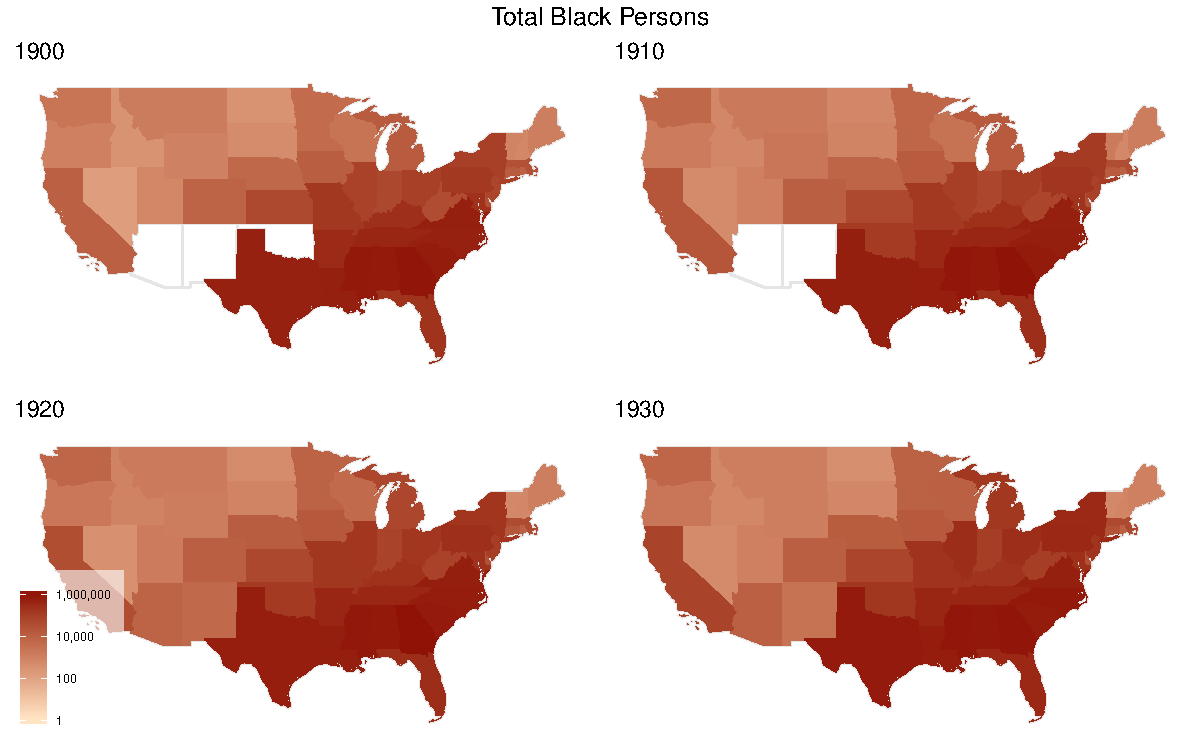
\includegraphics[width=.5\textwidth]{figure/map_1900s-1} \caption[Total number of black persons per state in 20th Century United States]{Total number of black persons per state in 20th Century United States.}\label{fig:map_1900s}
\end{figure}


\end{knitrout}



A period of growth and change can be seen at the turn of the 20th century as well, with a dramatic shift in the African American population out west to California and with the balance in the east and midwest shifting slightly further north (see \autoref{map_1900s}). Although the highest density of colored persons is still in the southern states, we can see that of a northern migration is taking place.

\section*{Conclusion}
The decennial census is a rich source of historical information. We have built a tool that can help extract and visualize that information to, for example, understand how demographic attributes of the U.S. population have changed over time.

Although there is no county-level information available and the data for the census browser go only through 1960, users are able to efficiently explore variables of interest at different time points in U.S. history and tell a visual story about a growing nation and a changing population. This connectivity across years and ability to assess what information was available when, all in one browser, have the potential to save time and effort of researchers interested in delving into United States history.

The structure of our browsers also helps determine not only the variables that are available in a given year, but also where information is missing for some states on a particular variable. Finding these differences is easier when all relevant variables are combined in one data frame, which can be summarized and searched all at one time.
%----------------------------------------------------------------------------------------
%	REFERENCE LIST
%----------------------------------------------------------------------------------------
\bibliographystyle{abbrv}
\bibliography{bibliography}
\section*{Further Reading}


%----------------------------------------------------------------------------------------

\end{document}
